%%%%%%%%%%%%%%%%%%%%%%%%%%%%%%%%%%%%%%%%%%%%%%%%%%%%%%%%%%%%%%%%%%%%%%%%%%%

\documentclass{article}

\usepackage{mathptmx}
\usepackage{tikz}
\usetikzlibrary{external}
\tikzexternalize{model}

%% We default to Times.
\renewcommand{\rmdefault}{ptm}
\renewcommand{\ttdefault}{pcr}
%% enable Times/Palatino main text font
\normalfont\selectfont

\begin{document}
%%
%% No page numbering.
\clearpage
\thispagestyle{empty}
%%
\begin{figure}
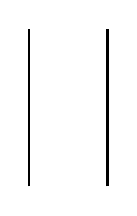
\begin{tikzpicture}[
  lineDecorate/.style={-,thick},%%
  nodeDecorate/.style={inner sep=0pt}%%
]
%% Global variables.
\pgfmathsetmacro{\Xax}{0}
\pgfmathsetmacro{\Xay}{2}
%%
%% Left-most window.
\draw[lineDecorate] (0,0) edge (\Xax,\Xay);
\draw[lineDecorate] (1,0) edge (1,2);
\end{tikzpicture}
\end{figure}

\end{document}
